\documentclass{article}
\usepackage{booktabs}
\usepackage{hyperref}
\usepackage{listings}
\usepackage{longtable}
\usepackage{tikz}
\begin{document}
\section*{Common package fixture}
\href{https://example.com}{A hyperlink}

\begin{longtable}{lr}
\toprule
Item & Value \\
\midrule
Alpha & 1 \\
Beta & 2 \\
\bottomrule
\end{longtable}

\begin{lstlisting}[language=Python]
answer = 42
\end{lstlisting}

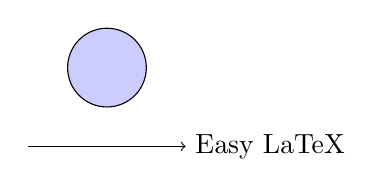
\begin{tikzpicture}
  \draw[->] (0,0) -- (2,0) node[right]{Easy LaTeX};
  \draw[fill=blue!20] (1,1) circle (0.5);
\end{tikzpicture}
\end{document}
